We introduce an automated testing service integrated in PaaS.
%
Developers write layered parameterized tests (LPTs) and upload them with the cloud application to be executed by the test service.  The service uses LPTs to automatically generate application inputs (e.g., web requests and persistent data) that exercise the application layers of interest.  The developer writes LPTs by specifying the structure of the application inputs and a target property to be checked.

\paragraph{Developer Workflow}

\begin{figure}
  \centering
  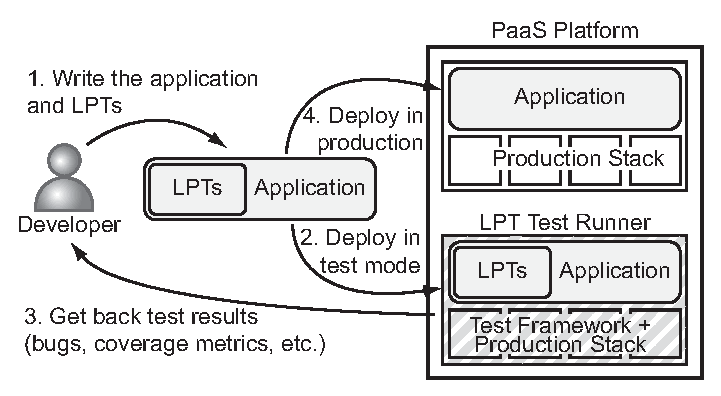
\includegraphics[width=0.8\textwidth]{paas/figures/developer-flow}
  \caption{Development flow for using a PaaS-integrated testing
    service.}
  \label{fig:development-flow}
\end{figure}

Figure~\ref{fig:development-flow} illustrates the workflow of a developer using our testing service.
%
The developer writes layered parameterized tests using a platform-provided testing API (step 1). She then deploys the app in test mode, which invokes the LPT test runner of the PaaS (step 2). This test runner is responsible for generating and running the individual test cases from the LPT, and it returns test results back to the developer (step 3). The develop-deploy-test cycle continues until the code is ready to be deployed in production (step 4).

% Might be misleading - the onion tests are much more powerful
% , and existing xUnit tests can be converted to onion tests.

%---------------------------------------------------------------------------
\paragraph{Layered Parameterized Tests}

An LPT specifies a family of executions (or, equivalently, classes of inputs) plus a set of properties (expressed as assertions) that are expected to hold for all these executions.
%
The specified family of executions can be large or even infinite; still, the test runner can often efficiently check whether the property is guaranteed to hold for the entire family (we give more details on the symbolic execution-based mechanism in Section~\ref{sec:paas:layeredsymbex}).  A traditional unit test can be seen as a special case of an LPT for which the input is fixed and any provided assertions are checked on a single execution only.

\begin{figure}
  \centering
  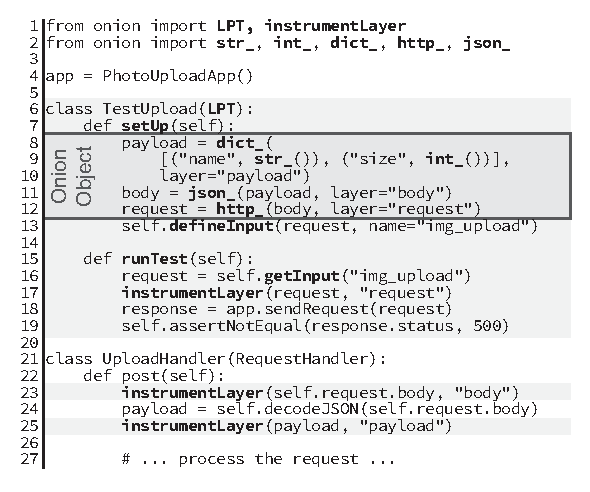
\includegraphics[width=0.7\textwidth]{paas/figures/overlay}
  \caption[An LPT example in Python for a photo management application.]{An LPT example in Python for a photo management application.  Highlighted code is the test code written by developers.  Names in bold denote the LPT-specific API added to the standard Python unit test framework.}
  \label{fig:test-lpt}
\end{figure}

\looseness=-1 LPTs are defined by developers using a platform-provided API in the implementation language of the application (e.g., Python).  The testing API builds on the popular xUnit testing paradigm~\cite{xunit} and extends it with constructs to specify the structure of families of application inputs.  The API is easily integrated with existing testing fixtures and frameworks that developers use today.

We illustrate the structure of an LPT and how it is used by the test runner using the example LPT \codebit{TestUpload} shown in Figure~\ref{fig:test-lpt}, which tests the upload functionality of a photo management application.  Under the \codebit{/upload} URL, the application accepts POST requests containing a JSON-encoded dictionary describing photo information.  Figure~\ref{fig:http-packet} shows an example HTTP request for the application.

We assume that the app follows the structure given in Figure~\ref{fig:running-example}, that it is written in Python using a popular web framework like Django~\cite{py-django} or WebApp~\cite{webapp2}, and that it is deployed on a PaaS infrastructure like Google App Engine~\cite{google-gae} or Heroku~\cite{heroku}.  The web framework takes care of dispatching any POST request to the \codebit{/upload} application URL to the \codebit{post} method of the \codebit{UploadHandler} class (lines 21--27).
%
The \codebit{TestUpload} LPT checks that, for arbitrary upload requests, the server never returns an internal error (HTTP 500) in its response.

\begin{figure}
  \centering
  
\includegraphics[width=0.7\textwidth]{paas/figures/http-packet}
  \caption[An example HTTP request for the upload feature of a photo management application.]{An example HTTP request for the upload feature of the photo management application.  The text in bold denotes input processed by the application at various layers.}
  \label{fig:http-packet}
\end{figure}

The test runner uses the LPT to automatically generate application
input according to the following procedure:

\begin{enumerate}
% Step 1
\item The test runner invokes the \codebit{setUp} method (line~7),
  which declares the application inputs and their structure as
  \emph{onion objects} (described below) using the
  \codebit{defineInput} call at line~13.
% Step 2
\item Based on the onion objects, the test runner generates a default
  input for the application.
% Step 3
\item The test runner invokes \codebit{runTest}, which retrieves the
  concrete input generated by the test runner with a call to
  \codebit{getInput} (line~16).  In our example, the input is a web
  request, which is then sent to the application (line~18).  Behind
  the scenes, the web framework dispatches the request to the
  \codebit{post} method of \codebit{UploadHandler} (line~22).  When
  the handler finishes handling the request, a response object with a
  status code and body is returned.  In our example, the LPT checks
  that no internal error (HTTP 500) occurred during request handling
  (line~19).
% Step 4
\item Based on the information collected during the execution of
  \codebit{runTest} (described below), the test runner uses the onion
  objects to generate a new application input (available to the LPT
  through the \codebit{getInput} call) and goes back to step 3 for a
  new iteration.  
%
  Any assertion failures triggered by the generated inputs are
  reported to the developers.
\end{enumerate}
%
Note that the generation and execution of multiple inputs is well
suited for parallelization across multiple nodes in the cloud. This
allows to leverage the availability of additional nodes to reduce the
total testing time.

The test runner uses symbolic execution to generate new inputs (described in more detail in Section~\ref{sec:paas:layeredsymbex}). To generate inputs that exercise the application at specific layers, the test runner needs:
\begin{itemize}
\item the unwrapped application inputs for the current execution at the different application layers, provided by developers through annotations in the application source code; and
\item information about the input structure, provided by the LPT's onion objects.
\end{itemize}

\paragraph{Annotating Application Layers}

A web request traverses several processing layers in an application.  First, it is received as an HTTP packet string; second, it is decoded into a URL, a set of headers, and request a body; third, the body contents is decoded and processed. Depending on the application framework, processing can involve additional layers, e.g., for converting JSON representations to language objects.

The application layers process data at corresponding layers of the input data (the bold parts of the HTTP request in Figure~\ref{fig:http-packet}). For instance, the application typically maps the URL to a request handler, checks the headers for authentication information, and processes the body contents in the request handler code.

To expose the application input to the LPT as it is being processed at each layer, developers annotate the variables holding the input data structures in the application source code.  Three layers have been declared in Figure~\ref{fig:test-lpt}: the HTTP request at line~17, the request body at line~23, and the JSON payload extracted from the body at line~25.  The \codebit{instrumentLayer} call attaches a layer name to a variable. Similar to assertion statements, the call is active when executed as part of a test invocation, but disabled in production, where the LPTs are not used.  For a typical web stack, only about three layers have to be annotated for each request handler, keeping the required effort on the developer side low.


%---------------------------------------------------------------------------
\paragraph{Onion Objects}

An \emph{onion object} is a data structure that describes the representations of the application input as it traverses multiple processing layers.  The onion object (i) enables more convenient assertion-writing by directly exposing the data layers, and (ii) enables automated test generation to focus on specific layers of the application. Onion objects are needed to specify the application inputs for onion tests, but they can also be used to store output as the cloud application constructs a response in layers.

The framed area in Figure~\ref{fig:test-lpt} shows the onion object for our running example.  The structure consists of a set of \emph{onion nodes} (the identifiers ending in an underscore) connected in a nested structure.  There is one onion node for each layer and one for each input structure or value that is supposed to be generated automatically by the test engine.  The abstraction level is declared using the \codebit{layer} parameter passed to the node constructor and matches one of the layers annotated in the code.  Structures and values can be nested within the same layer.  For example, the dictionary structure on lines~8--10 has constant keys and wildcard values of type \codebit{str\_} and \codebit{int\_}, which mimic the standard string and integer types.

\paragraph{Checking Properties}

LPTs express application properties through standard xUnit assertion statements (line~19 in the example).  Through the dynamic test generation mechanism explained in Section~\ref{sec:paas:layeredsymbex}, the test runner actively attempts to generate inputs that cause an assertion to be violated. Each generated test input not failing the assertion serves as a witness for an entire equivalence class of inputs that cannot violate the assertion.
%
When an assertion does fail, the input that caused the failure is reported back to the developer.

To allow input variables at each layer to be used in assertions, each onion node offers a \codebit{value} property that refers to the value matched in the current test execution (not shown in the example).

%%% Local Variables: 
%%% mode: latex
%%% eval: (visual-line-mode)
%%% fill-column: 1000000
%%% TeX-master: "main"
%%% End:
